\documentclass[letterpaper,12pt]{article}
\usepackage[margin=14mm,top=18mm,bottom=17mm,headheight=14pt]{geometry}
\pdfmapfile{+cm.map}\pdfmapfile{+cmextra.map}
\usepackage{tikz,fancyhdr,amsmath,amssymb}
\usetikzlibrary{arrows.meta,patterns}
\pagestyle{fancy}\fancyhf{}\renewcommand{\headrulewidth}{0pt}
\fancyhead[L]{\small Week 48 / Inside and outside covers / Grades 4--5}
\fancyfoot[L]{\small Bellingham Math Circle / Week 48 / F48-45-v2}
\fancyfoot[R]{\small\thepage}
\setlength{\parindent}{0pt}\setlength{\parskip}{0pt}
\begin{document}
\noindent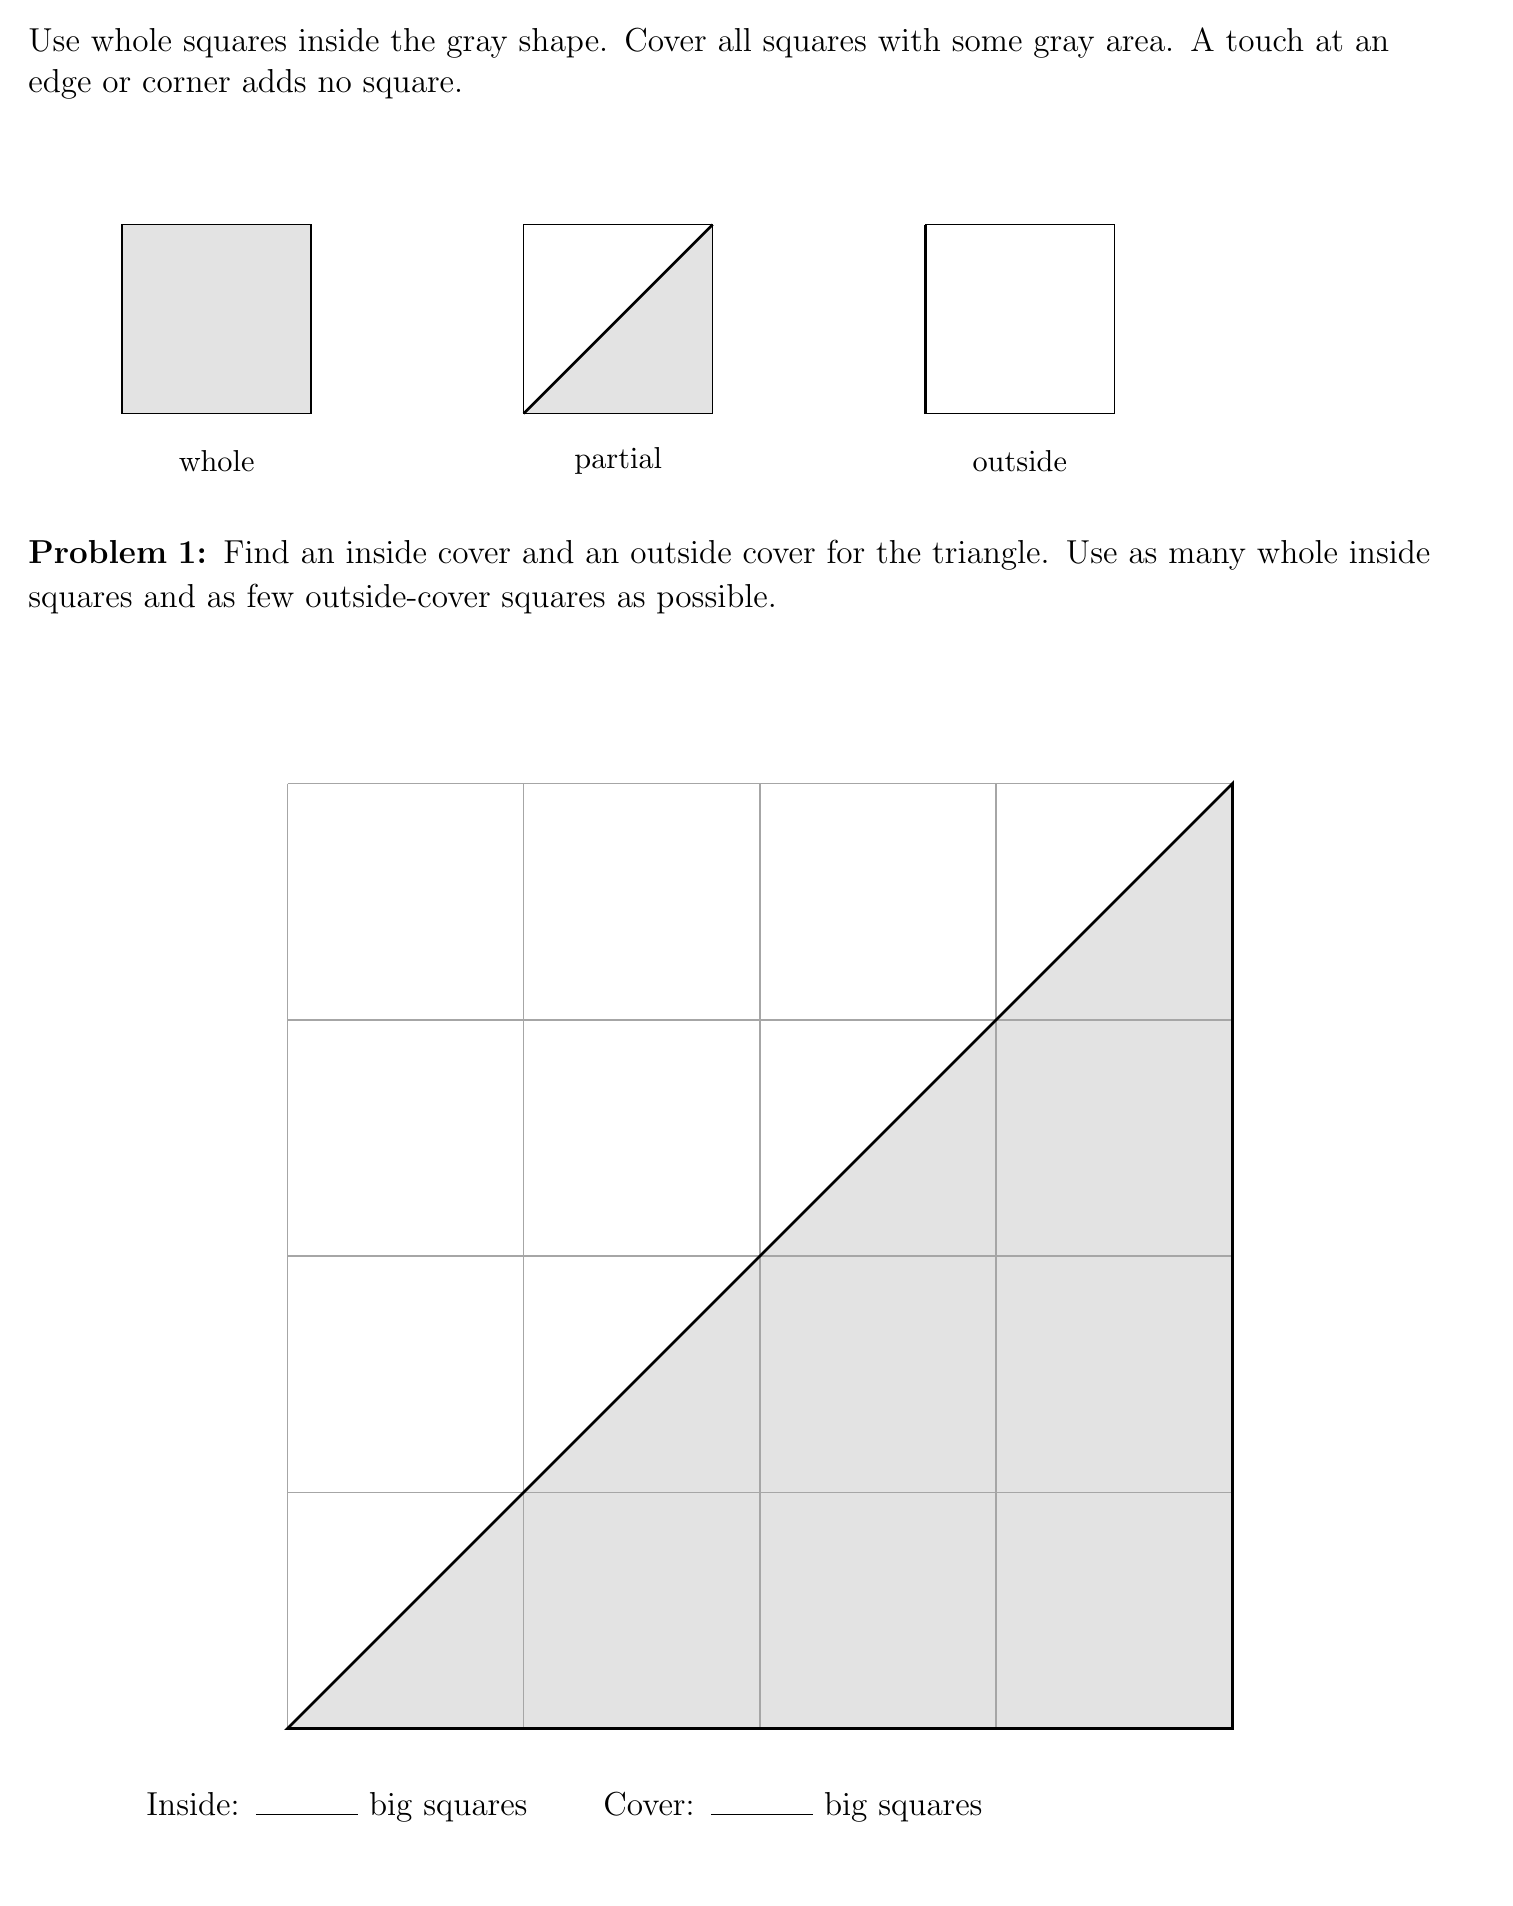
\begin{tikzpicture}[x=1mm,y=-1mm,line width=.5pt]
\path[use as bounding box] (0,0) rectangle (185,235);
\node[anchor=north west,inner sep=0pt,text width=180mm,font=\fontsize{12}{15}\selectfont] at (0,0) {Use whole squares inside the gray shape. Cover all squares with some gray area. A touch at an edge or corner adds no square.};
\draw[fill=gray!22] (12,25) rectangle ++(24,24);
\node[anchor=center,inner sep=1pt,font=\fontsize{11}{13}\selectfont] at (24,55) {whole};
\fill[gray!22] (63,49)--(87,49)--(87,25)--cycle;
\draw[] (63,25) rectangle ++(24,24);
\draw[line width=1pt] (63,49) -- (87,25);
\node[anchor=center,inner sep=1pt,font=\fontsize{11}{13}\selectfont] at (75,55) {partial};
\draw[] (114,25) rectangle ++(24,24);
\draw[line width=1.2pt] (114,25) -- (114,49);
\node[anchor=center,inner sep=1pt,font=\fontsize{11}{13}\selectfont] at (126,55) {outside};
\node[anchor=north west,inner sep=0pt,text width=180mm,font=\fontsize{13}{16}\selectfont] at (0,65) {\textbf{Problem 1:} Find an inside cover and an outside cover for the triangle. Use as many whole inside squares and as few outside-cover squares as possible.};
\fill[gray!22] (33.0,216.0) -- (153.0,216.0) -- (153.0,96.0) -- cycle;
\draw[gray!70] (33.0,96) -- (33.0,216);
\draw[gray!70] (33,96.0) -- (153,96.0);
\draw[gray!70] (63.0,96) -- (63.0,216);
\draw[gray!70] (33,126.0) -- (153,126.0);
\draw[gray!70] (93.0,96) -- (93.0,216);
\draw[gray!70] (33,156.0) -- (153,156.0);
\draw[gray!70] (123.0,96) -- (123.0,216);
\draw[gray!70] (33,186.0) -- (153,186.0);
\draw[gray!70] (153.0,96) -- (153.0,216);
\draw[gray!70] (33,216.0) -- (153,216.0);
\draw[line width=1pt] (33.0,216.0) -- (153.0,216.0) -- (153.0,96.0) -- cycle;
\node[anchor=north west,inner sep=0pt,text width=180mm,font=\fontsize{12}{15}\selectfont] at (15,224) {Inside: \rule{13mm}{.3pt} big squares \qquad Cover: \rule{13mm}{.3pt} big squares};
\end{tikzpicture}
\newpage
\noindent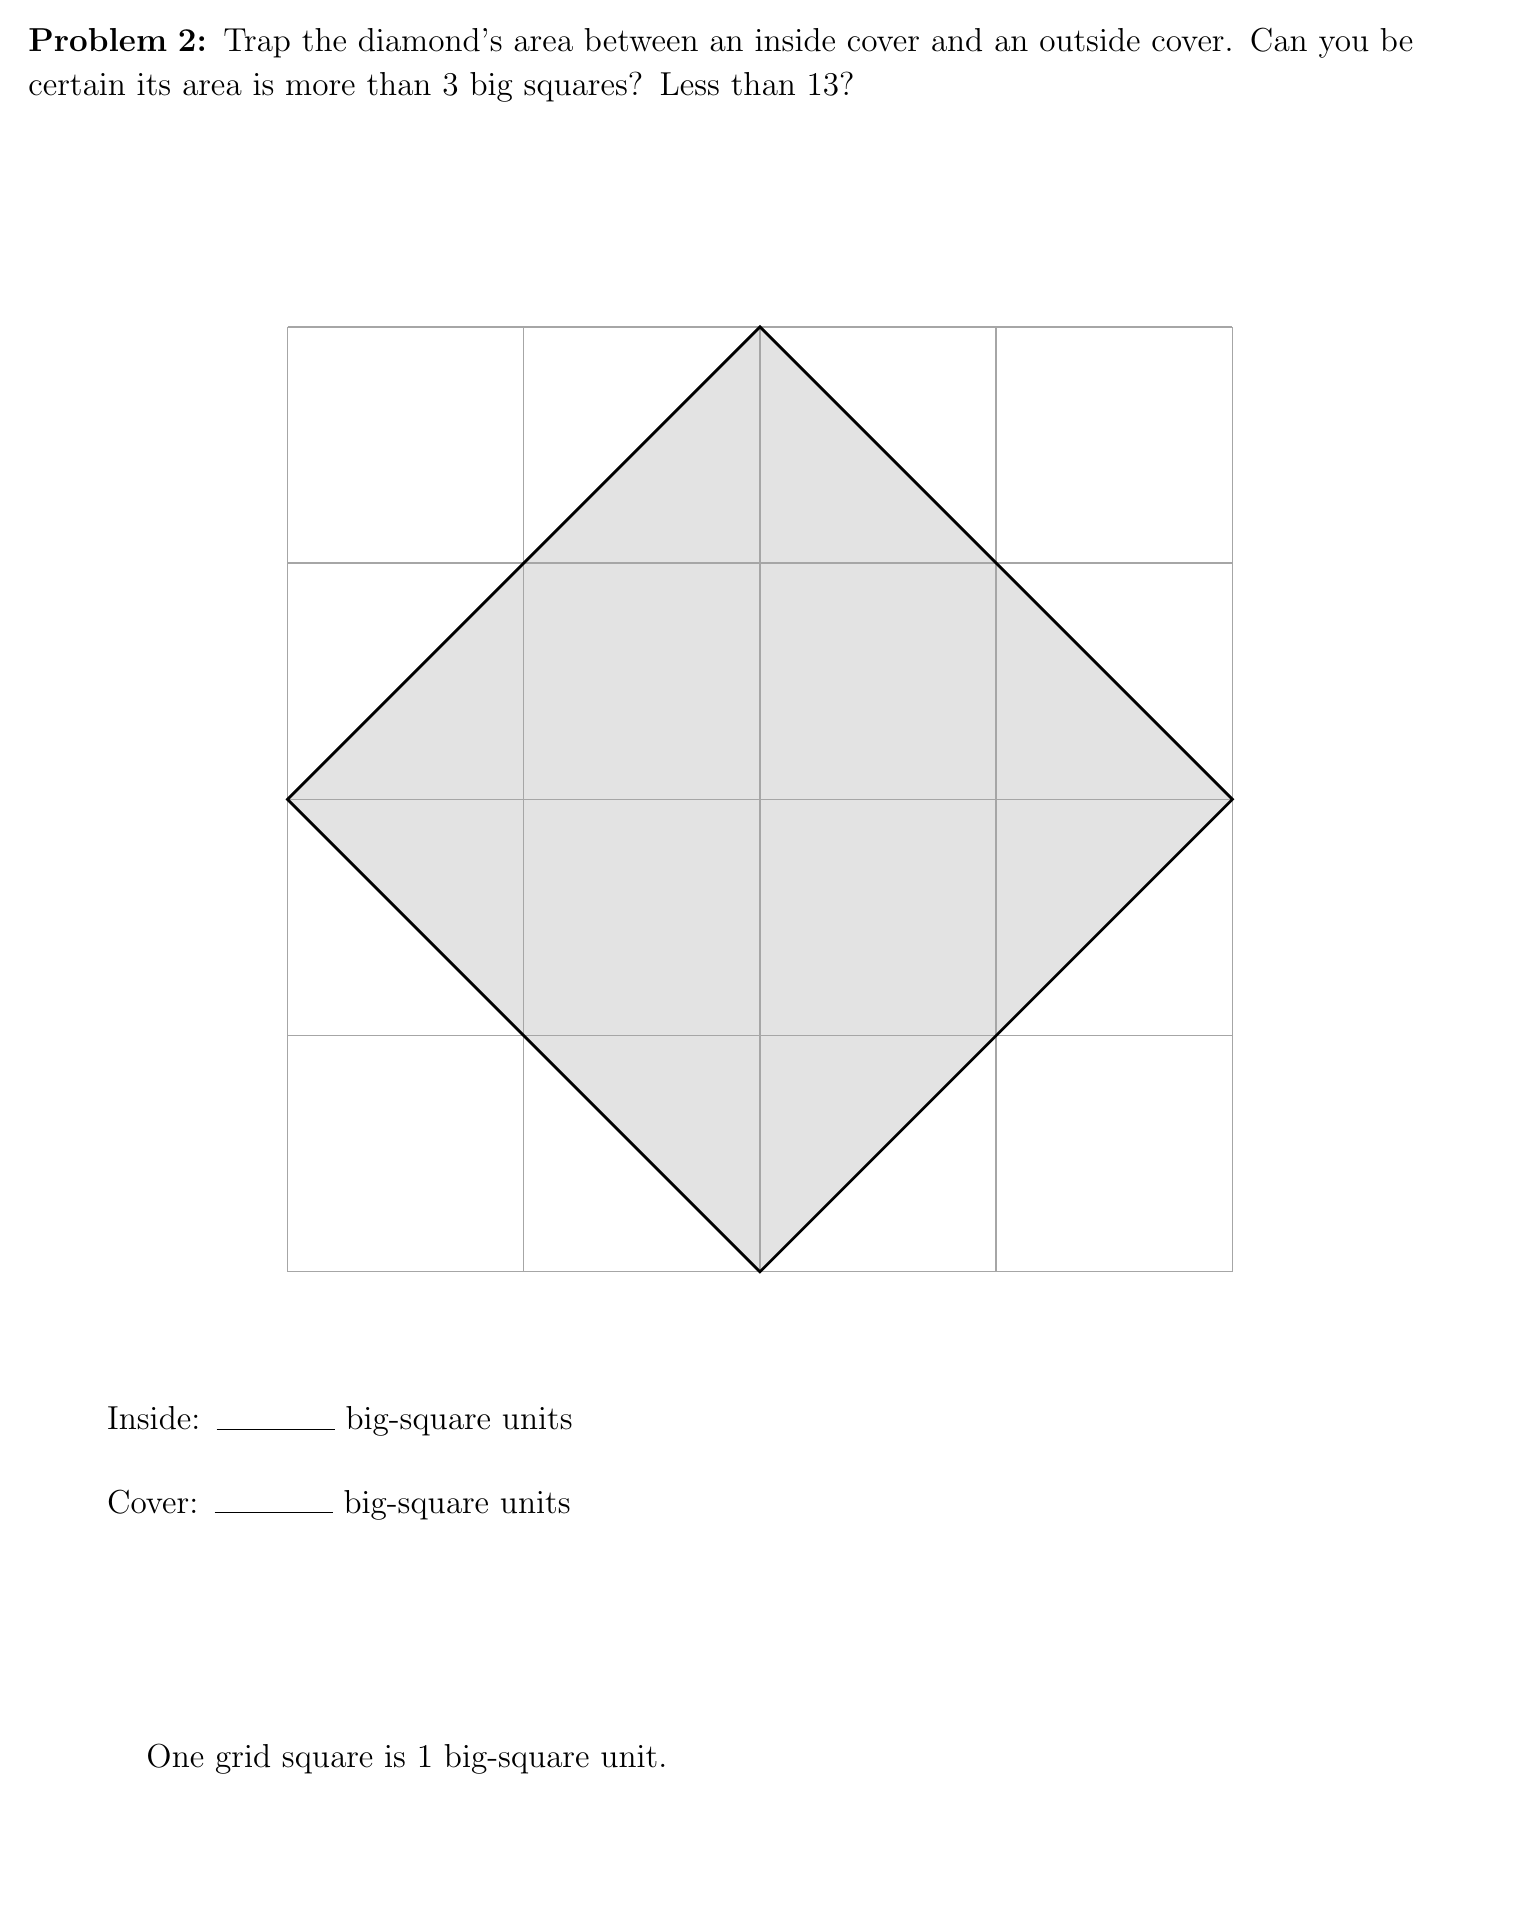
\begin{tikzpicture}[x=1mm,y=-1mm,line width=.5pt]
\path[use as bounding box] (0,0) rectangle (185,235);
\node[anchor=north west,inner sep=0pt,text width=180mm,font=\fontsize{13}{16}\selectfont] at (0,0) {\textbf{Problem 2:} Trap the diamond's area between an inside cover and an outside cover. Can you be certain its area is more than 3 big squares? Less than 13?};
\fill[gray!22] (33.0,98.0) -- (93.0,38.0) -- (153.0,98.0) -- (93.0,158.0) -- cycle;
\draw[gray!70] (33.0,38) -- (33.0,158);
\draw[gray!70] (33,38.0) -- (153,38.0);
\draw[gray!70] (63.0,38) -- (63.0,158);
\draw[gray!70] (33,68.0) -- (153,68.0);
\draw[gray!70] (93.0,38) -- (93.0,158);
\draw[gray!70] (33,98.0) -- (153,98.0);
\draw[gray!70] (123.0,38) -- (123.0,158);
\draw[gray!70] (33,128.0) -- (153,128.0);
\draw[gray!70] (153.0,38) -- (153.0,158);
\draw[gray!70] (33,158.0) -- (153,158.0);
\draw[line width=1pt] (33.0,98.0) -- (93.0,38.0) -- (153.0,98.0) -- (93.0,158.0) -- cycle;
\node[anchor=north west,inner sep=0pt,text width=170mm,font=\fontsize{13}{16}\selectfont] at (10,175) {Inside: \rule{15mm}{.3pt} big-square units\\[5mm]Cover: \rule{15mm}{.3pt} big-square units};
\node[anchor=north west,inner sep=0pt,text width=180mm,font=\fontsize{12}{15}\selectfont] at (15,218) {One grid square is 1 big-square unit.};
\end{tikzpicture}
\newpage
\noindent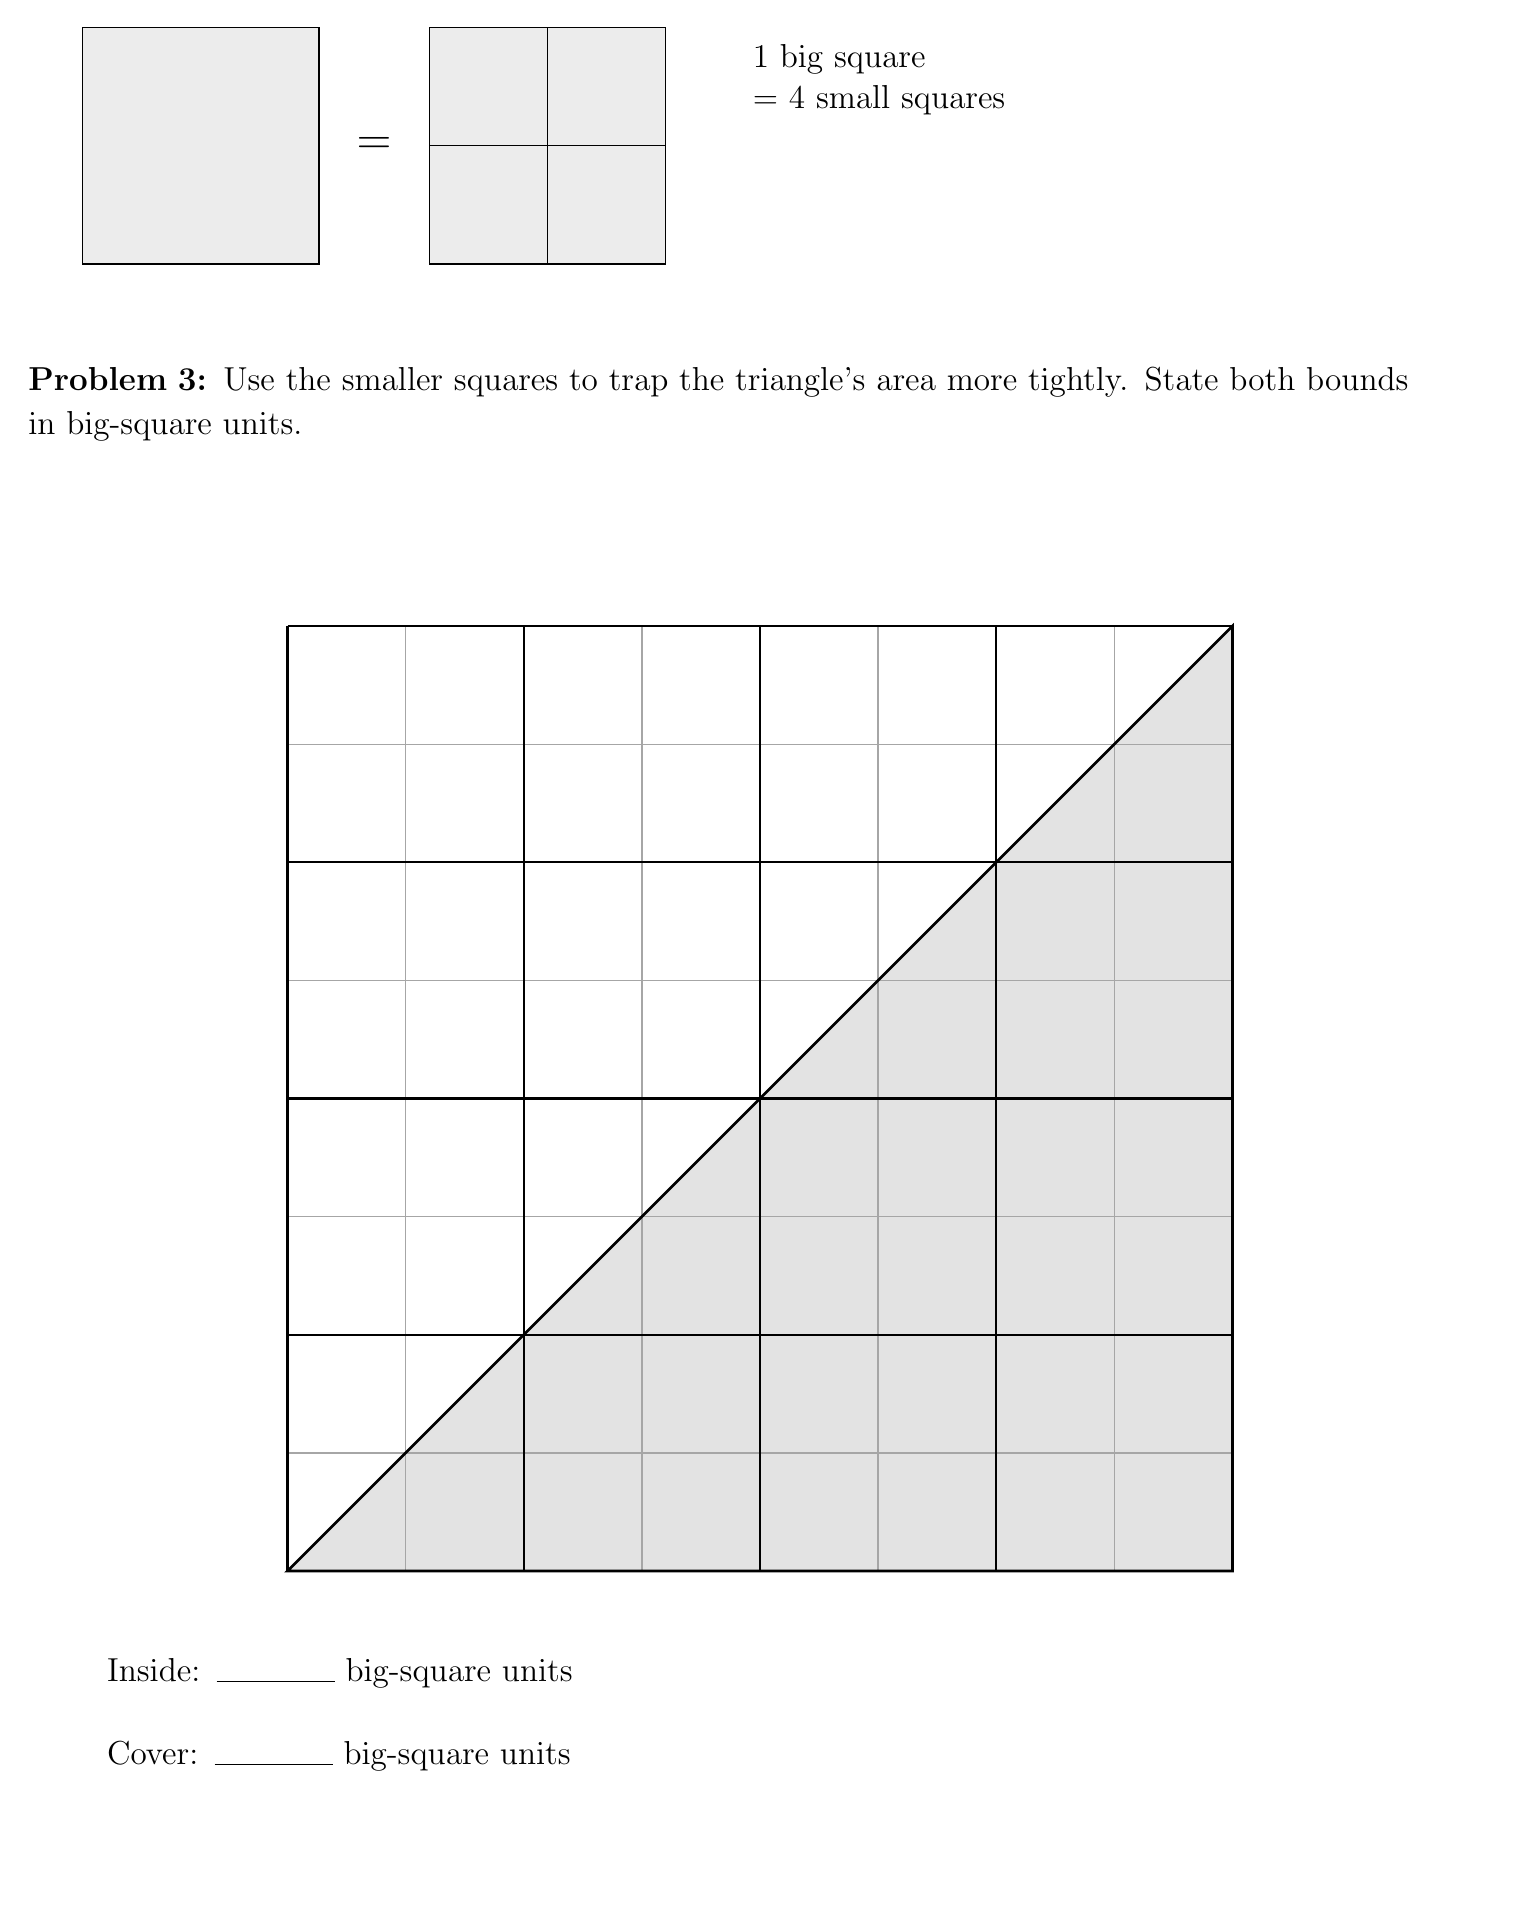
\begin{tikzpicture}[x=1mm,y=-1mm,line width=.5pt]
\path[use as bounding box] (0,0) rectangle (185,235);
\draw[fill=gray!15] (7,0) rectangle ++(30,30);
\node[anchor=center,inner sep=1pt,font=\fontsize{16}{18}\selectfont] at (44,15) {=};
\draw[fill=gray!15] (51,0) rectangle ++(15,15);
\draw[fill=gray!15] (51,15) rectangle ++(15,15);
\draw[fill=gray!15] (66,0) rectangle ++(15,15);
\draw[fill=gray!15] (66,15) rectangle ++(15,15);
\node[anchor=north west,inner sep=0pt,text width=83mm,font=\fontsize{12}{15}\selectfont] at (92,2) {1 big square\\ = 4 small squares};
\node[anchor=north west,inner sep=0pt,text width=180mm,font=\fontsize{13}{16}\selectfont] at (0,43) {\textbf{Problem 3:} Use the smaller squares to trap the triangle's area more tightly. State both bounds in big-square units.};
\fill[gray!22] (33.0,196.0) -- (153.0,196.0) -- (153.0,76.0) -- cycle;
\draw[gray!70] (33.0,76) -- (33.0,196);
\draw[gray!70] (33,76.0) -- (153,76.0);
\draw[gray!70] (48.0,76) -- (48.0,196);
\draw[gray!70] (33,91.0) -- (153,91.0);
\draw[gray!70] (63.0,76) -- (63.0,196);
\draw[gray!70] (33,106.0) -- (153,106.0);
\draw[gray!70] (78.0,76) -- (78.0,196);
\draw[gray!70] (33,121.0) -- (153,121.0);
\draw[gray!70] (93.0,76) -- (93.0,196);
\draw[gray!70] (33,136.0) -- (153,136.0);
\draw[gray!70] (108.0,76) -- (108.0,196);
\draw[gray!70] (33,151.0) -- (153,151.0);
\draw[gray!70] (123.0,76) -- (123.0,196);
\draw[gray!70] (33,166.0) -- (153,166.0);
\draw[gray!70] (138.0,76) -- (138.0,196);
\draw[gray!70] (33,181.0) -- (153,181.0);
\draw[gray!70] (153.0,76) -- (153.0,196);
\draw[gray!70] (33,196.0) -- (153,196.0);
\draw[line width=.8pt] (33.0,76) -- (33.0,196);
\draw[line width=.8pt] (33,76.0) -- (153,76.0);
\draw[line width=.8pt] (63.0,76) -- (63.0,196);
\draw[line width=.8pt] (33,106.0) -- (153,106.0);
\draw[line width=.8pt] (93.0,76) -- (93.0,196);
\draw[line width=.8pt] (33,136.0) -- (153,136.0);
\draw[line width=.8pt] (123.0,76) -- (123.0,196);
\draw[line width=.8pt] (33,166.0) -- (153,166.0);
\draw[line width=.8pt] (153.0,76) -- (153.0,196);
\draw[line width=.8pt] (33,196.0) -- (153,196.0);
\draw[line width=1pt] (33.0,196.0) -- (153.0,196.0) -- (153.0,76.0) -- cycle;
\node[anchor=north west,inner sep=0pt,text width=170mm,font=\fontsize{13}{16}\selectfont] at (10,207) {Inside: \rule{15mm}{.3pt} big-square units\\[5mm]Cover: \rule{15mm}{.3pt} big-square units};
\end{tikzpicture}
\newpage
\noindent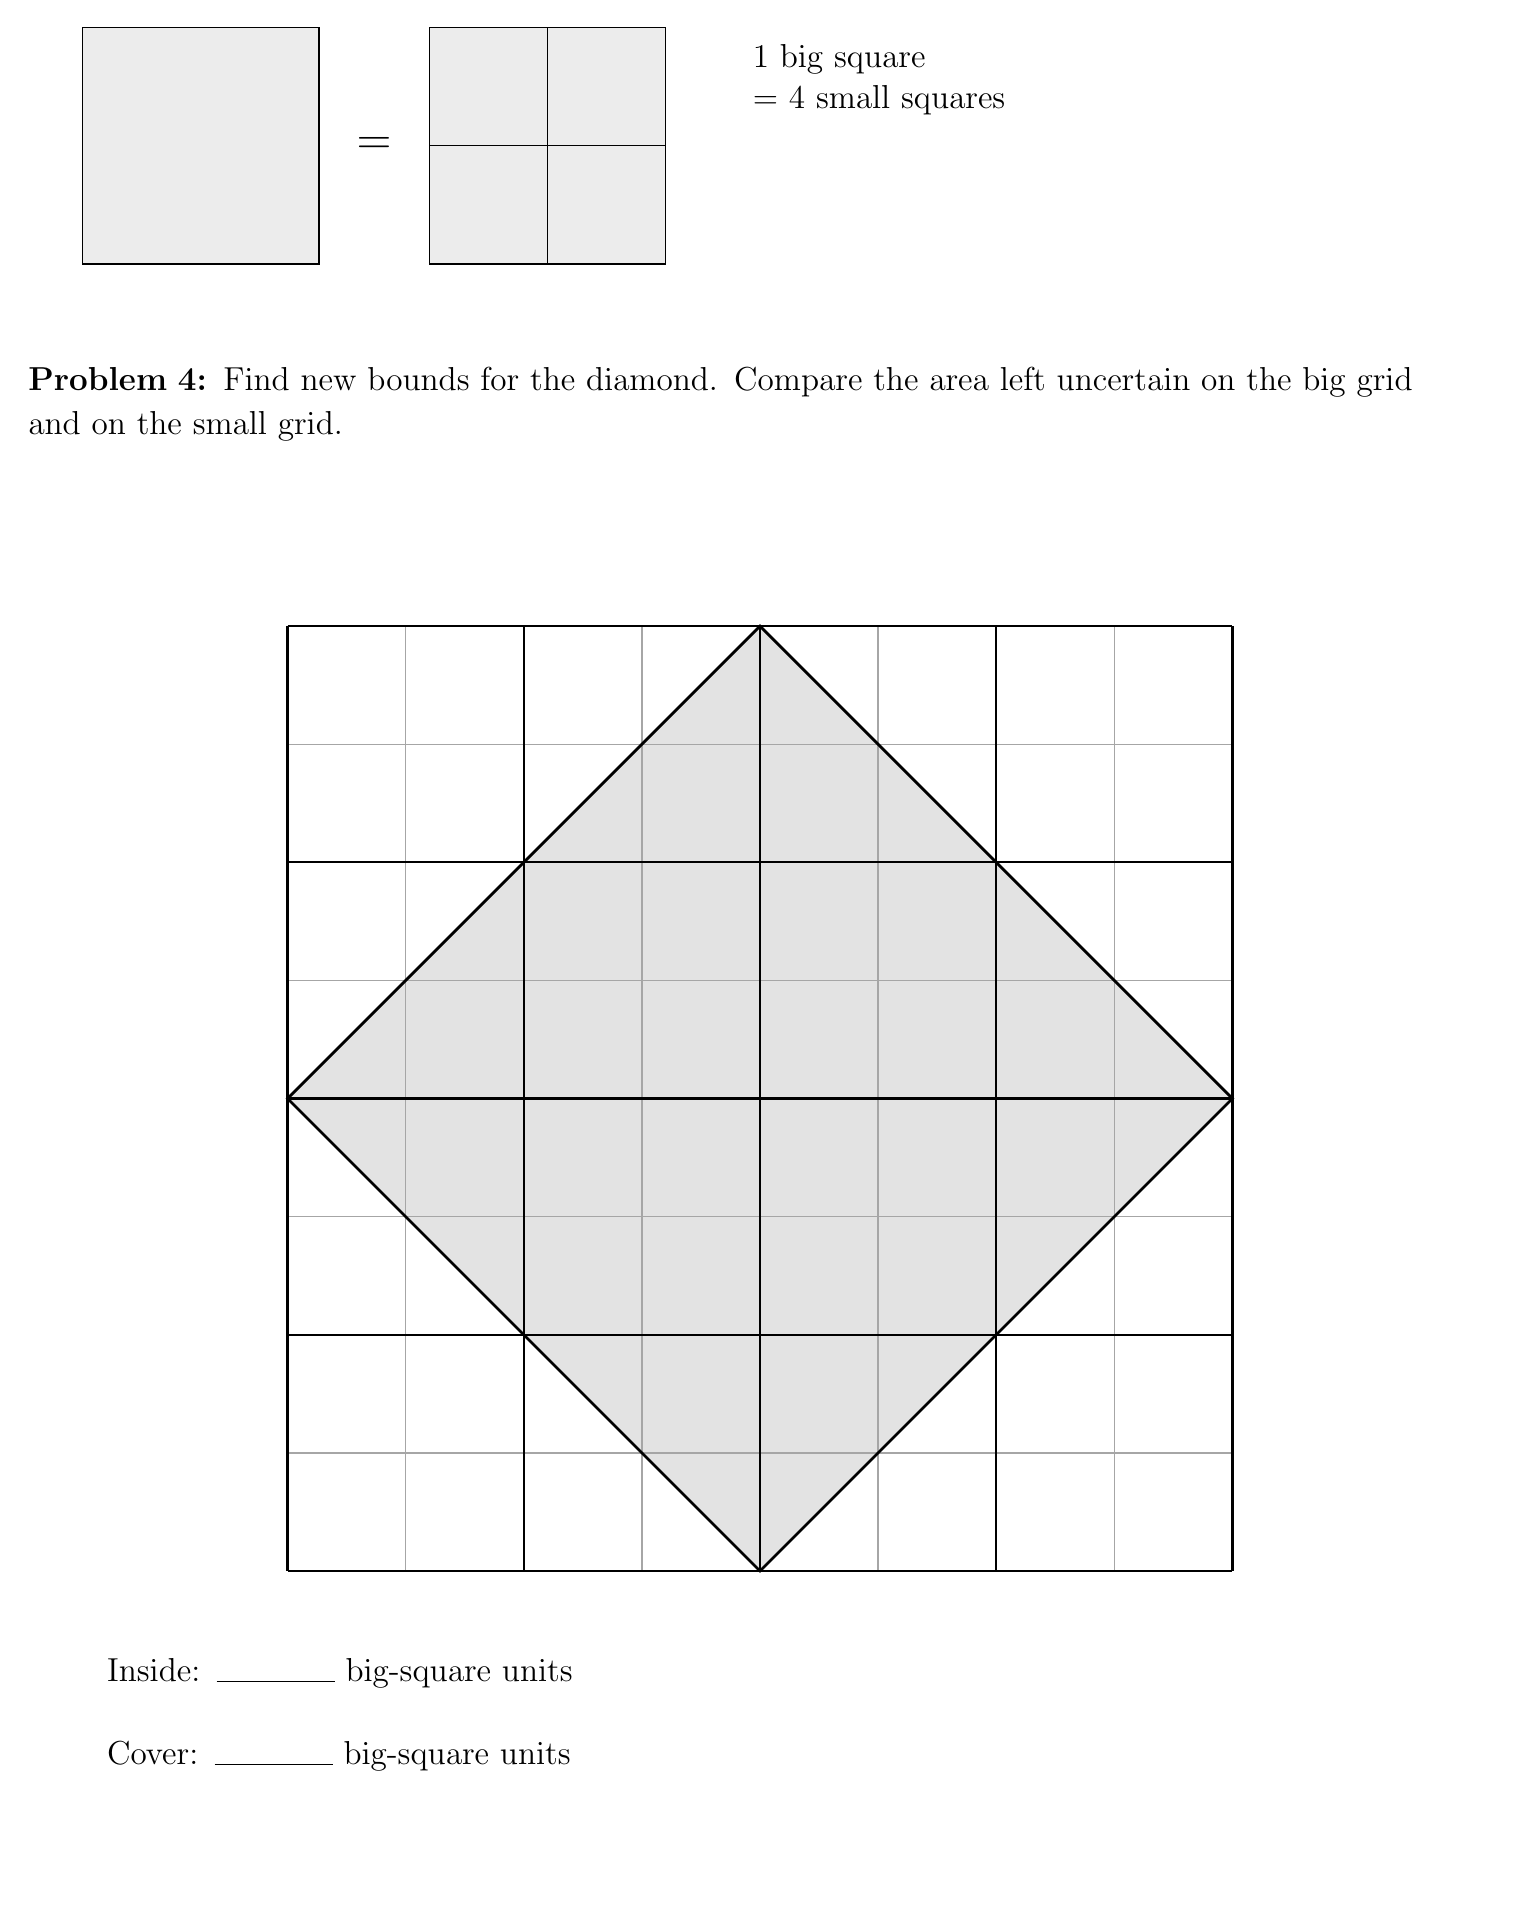
\begin{tikzpicture}[x=1mm,y=-1mm,line width=.5pt]
\path[use as bounding box] (0,0) rectangle (185,235);
\draw[fill=gray!15] (7,0) rectangle ++(30,30);
\node[anchor=center,inner sep=1pt,font=\fontsize{16}{18}\selectfont] at (44,15) {=};
\draw[fill=gray!15] (51,0) rectangle ++(15,15);
\draw[fill=gray!15] (51,15) rectangle ++(15,15);
\draw[fill=gray!15] (66,0) rectangle ++(15,15);
\draw[fill=gray!15] (66,15) rectangle ++(15,15);
\node[anchor=north west,inner sep=0pt,text width=83mm,font=\fontsize{12}{15}\selectfont] at (92,2) {1 big square\\ = 4 small squares};
\node[anchor=north west,inner sep=0pt,text width=180mm,font=\fontsize{13}{16}\selectfont] at (0,43) {\textbf{Problem 4:} Find new bounds for the diamond. Compare the area left uncertain on the big grid and on the small grid.};
\fill[gray!22] (33.0,136.0) -- (93.0,76.0) -- (153.0,136.0) -- (93.0,196.0) -- cycle;
\draw[gray!70] (33.0,76) -- (33.0,196);
\draw[gray!70] (33,76.0) -- (153,76.0);
\draw[gray!70] (48.0,76) -- (48.0,196);
\draw[gray!70] (33,91.0) -- (153,91.0);
\draw[gray!70] (63.0,76) -- (63.0,196);
\draw[gray!70] (33,106.0) -- (153,106.0);
\draw[gray!70] (78.0,76) -- (78.0,196);
\draw[gray!70] (33,121.0) -- (153,121.0);
\draw[gray!70] (93.0,76) -- (93.0,196);
\draw[gray!70] (33,136.0) -- (153,136.0);
\draw[gray!70] (108.0,76) -- (108.0,196);
\draw[gray!70] (33,151.0) -- (153,151.0);
\draw[gray!70] (123.0,76) -- (123.0,196);
\draw[gray!70] (33,166.0) -- (153,166.0);
\draw[gray!70] (138.0,76) -- (138.0,196);
\draw[gray!70] (33,181.0) -- (153,181.0);
\draw[gray!70] (153.0,76) -- (153.0,196);
\draw[gray!70] (33,196.0) -- (153,196.0);
\draw[line width=.8pt] (33.0,76) -- (33.0,196);
\draw[line width=.8pt] (33,76.0) -- (153,76.0);
\draw[line width=.8pt] (63.0,76) -- (63.0,196);
\draw[line width=.8pt] (33,106.0) -- (153,106.0);
\draw[line width=.8pt] (93.0,76) -- (93.0,196);
\draw[line width=.8pt] (33,136.0) -- (153,136.0);
\draw[line width=.8pt] (123.0,76) -- (123.0,196);
\draw[line width=.8pt] (33,166.0) -- (153,166.0);
\draw[line width=.8pt] (153.0,76) -- (153.0,196);
\draw[line width=.8pt] (33,196.0) -- (153,196.0);
\draw[line width=1pt] (33.0,136.0) -- (93.0,76.0) -- (153.0,136.0) -- (93.0,196.0) -- cycle;
\node[anchor=north west,inner sep=0pt,text width=170mm,font=\fontsize{13}{16}\selectfont] at (10,207) {Inside: \rule{15mm}{.3pt} big-square units\\[5mm]Cover: \rule{15mm}{.3pt} big-square units};
\end{tikzpicture}
\newpage
\noindent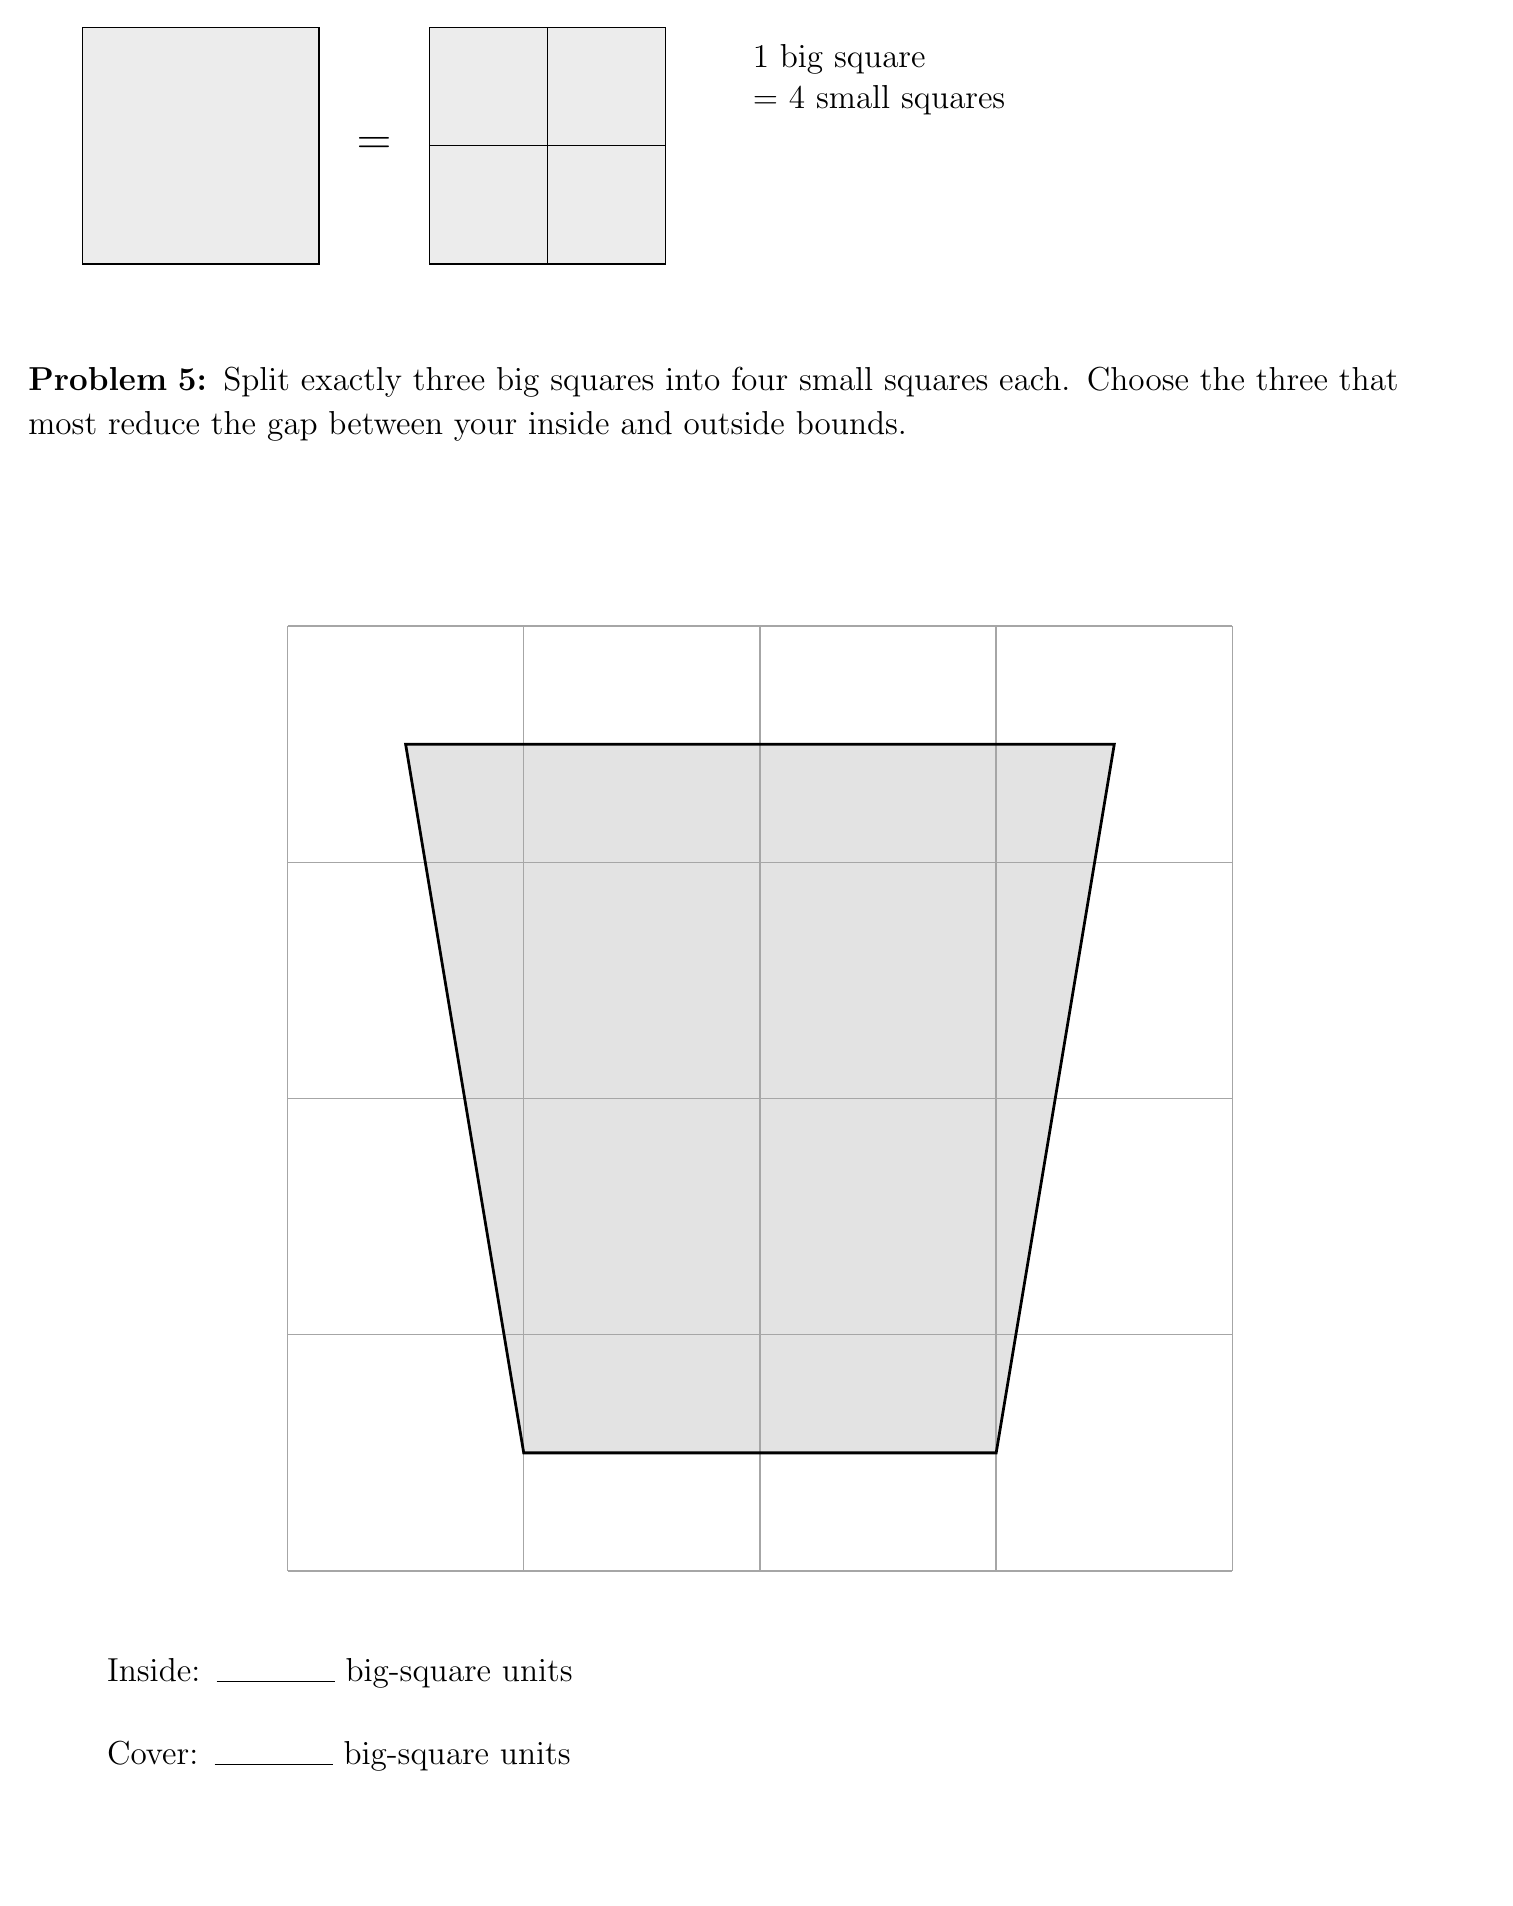
\begin{tikzpicture}[x=1mm,y=-1mm,line width=.5pt]
\path[use as bounding box] (0,0) rectangle (185,235);
\draw[fill=gray!15] (7,0) rectangle ++(30,30);
\node[anchor=center,inner sep=1pt,font=\fontsize{16}{18}\selectfont] at (44,15) {=};
\draw[fill=gray!15] (51,0) rectangle ++(15,15);
\draw[fill=gray!15] (51,15) rectangle ++(15,15);
\draw[fill=gray!15] (66,0) rectangle ++(15,15);
\draw[fill=gray!15] (66,15) rectangle ++(15,15);
\node[anchor=north west,inner sep=0pt,text width=83mm,font=\fontsize{12}{15}\selectfont] at (92,2) {1 big square\\ = 4 small squares};
\node[anchor=north west,inner sep=0pt,text width=180mm,font=\fontsize{13}{16}\selectfont] at (0,43) {\textbf{Problem 5:} Split exactly three big squares into four small squares each. Choose the three that most reduce the gap between your inside and outside bounds.};
\fill[gray!22] (48.0,91.0) -- (138.0,91.0) -- (123.0,181.0) -- (63.0,181.0) -- cycle;
\draw[gray!70] (33.0,76) -- (33.0,196);
\draw[gray!70] (33,76.0) -- (153,76.0);
\draw[gray!70] (63.0,76) -- (63.0,196);
\draw[gray!70] (33,106.0) -- (153,106.0);
\draw[gray!70] (93.0,76) -- (93.0,196);
\draw[gray!70] (33,136.0) -- (153,136.0);
\draw[gray!70] (123.0,76) -- (123.0,196);
\draw[gray!70] (33,166.0) -- (153,166.0);
\draw[gray!70] (153.0,76) -- (153.0,196);
\draw[gray!70] (33,196.0) -- (153,196.0);
\draw[line width=1pt] (48.0,91.0) -- (138.0,91.0) -- (123.0,181.0) -- (63.0,181.0) -- cycle;
\node[anchor=north west,inner sep=0pt,text width=170mm,font=\fontsize{13}{16}\selectfont] at (10,207) {Inside: \rule{15mm}{.3pt} big-square units\\[5mm]Cover: \rule{15mm}{.3pt} big-square units};
\end{tikzpicture}
\newpage
\noindent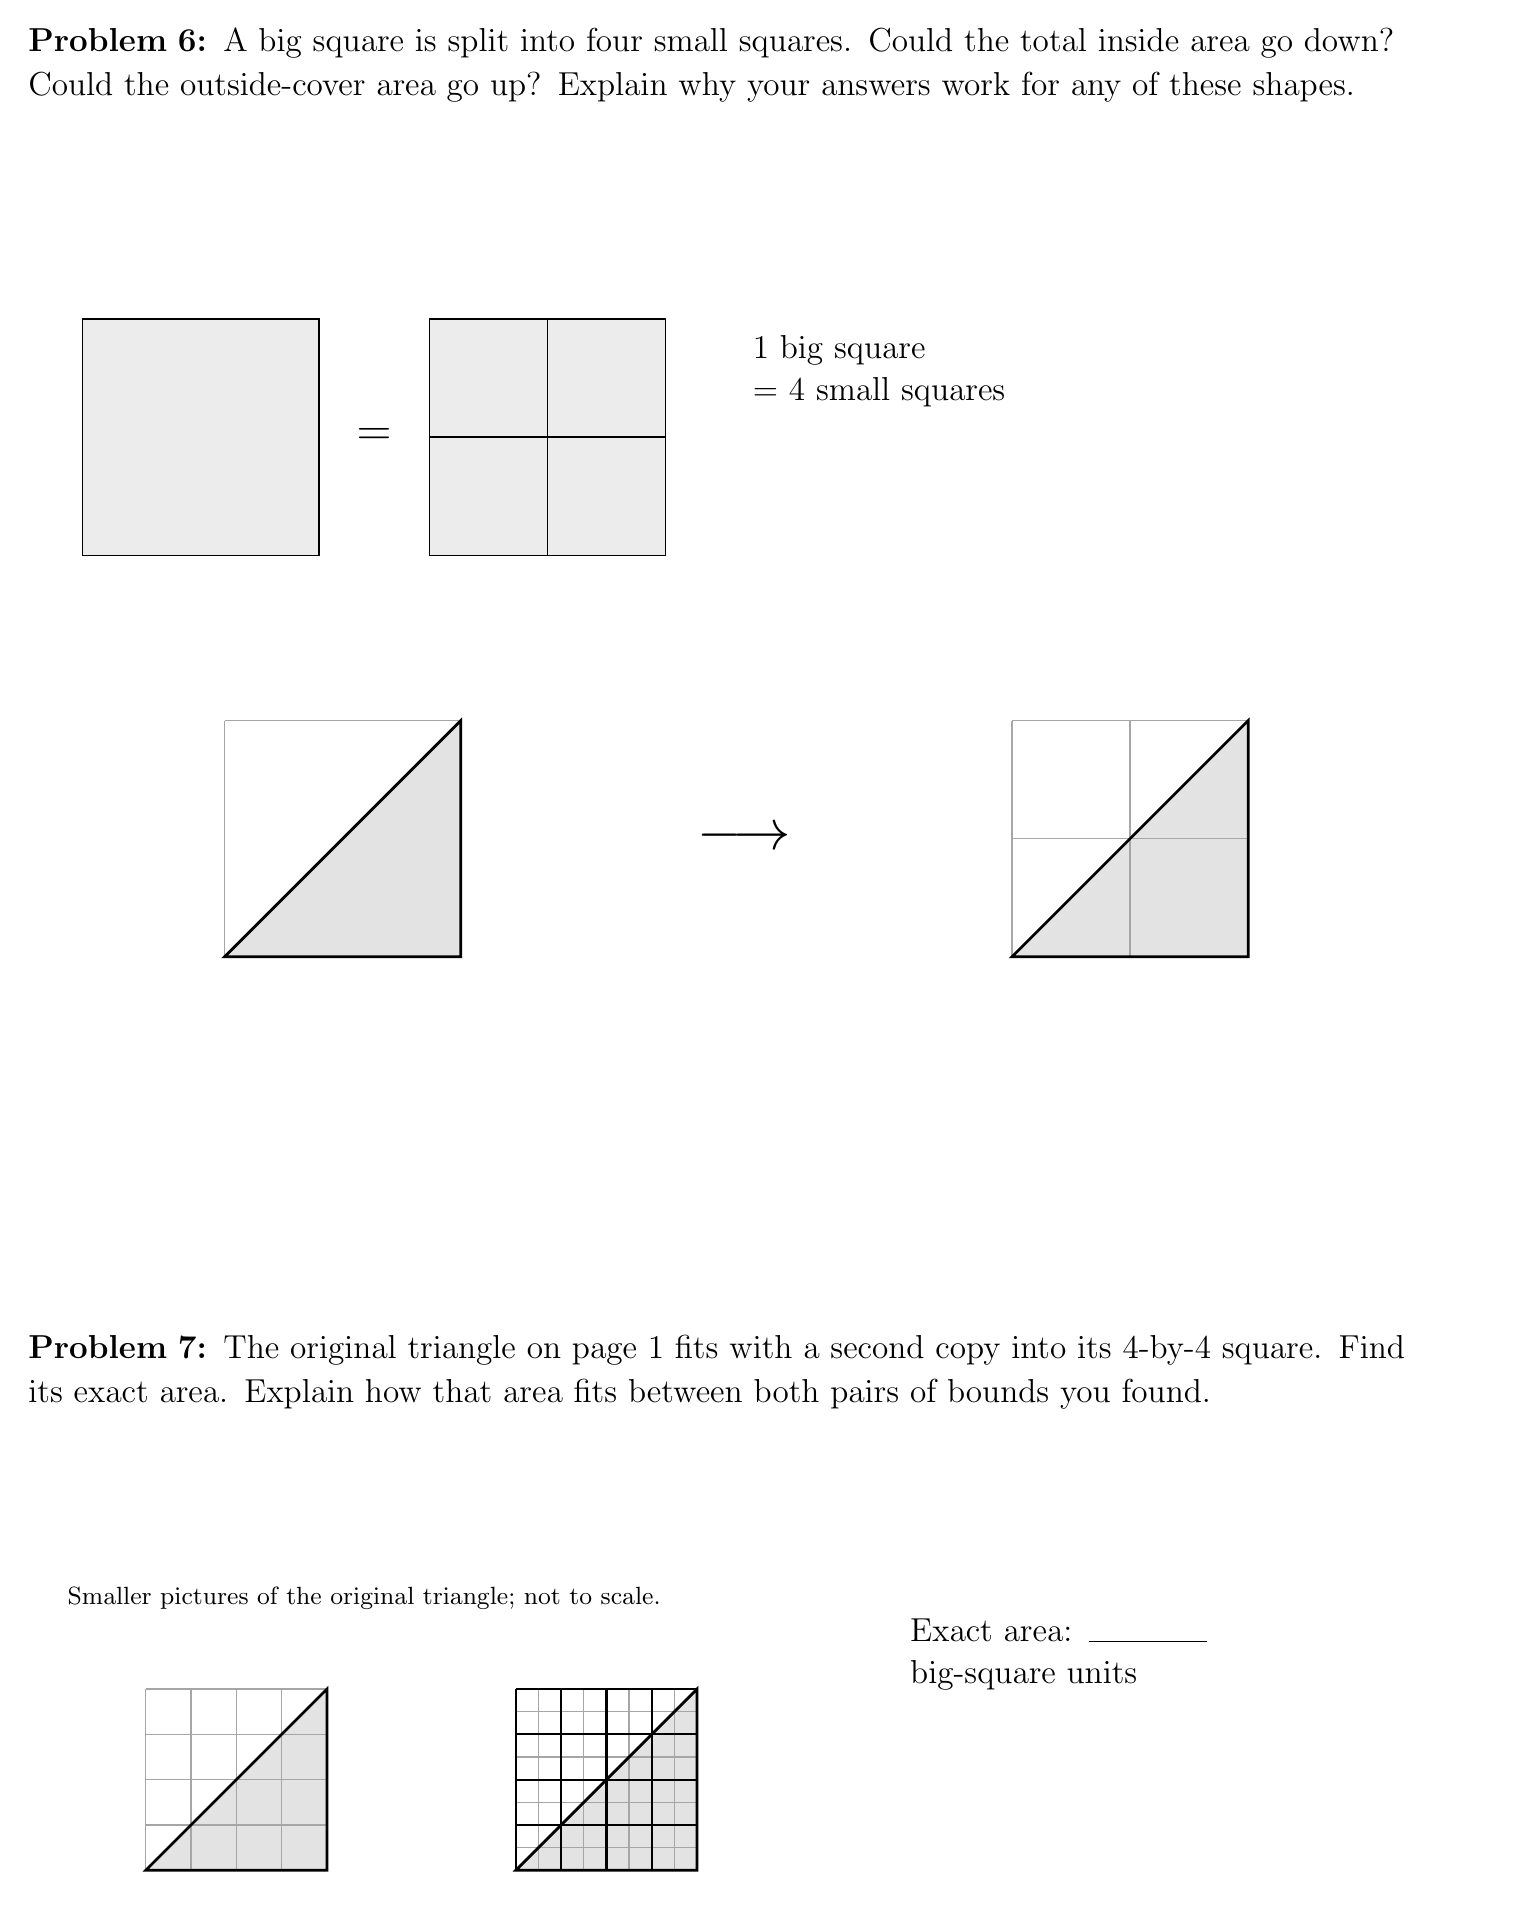
\begin{tikzpicture}[x=1mm,y=-1mm,line width=.5pt]
\path[use as bounding box] (0,0) rectangle (185,235);
\node[anchor=north west,inner sep=0pt,text width=180mm,font=\fontsize{13}{16}\selectfont] at (0,0) {\textbf{Problem 6:} A big square is split into four small squares. Could the total inside area go down? Could the outside-cover area go up? Explain why your answers work for any of these shapes.};
\draw[fill=gray!15] (7,37) rectangle ++(30,30);
\node[anchor=center,inner sep=1pt,font=\fontsize{16}{18}\selectfont] at (44,52) {=};
\draw[fill=gray!15] (51,37) rectangle ++(15,15);
\draw[fill=gray!15] (51,52) rectangle ++(15,15);
\draw[fill=gray!15] (66,37) rectangle ++(15,15);
\draw[fill=gray!15] (66,52) rectangle ++(15,15);
\node[anchor=north west,inner sep=0pt,text width=83mm,font=\fontsize{12}{15}\selectfont] at (92,39) {1 big square\\ = 4 small squares};
\fill[gray!22] (25.0,118.0) -- (55.0,118.0) -- (55.0,88.0) -- cycle;
\draw[gray!70] (25.0,88) -- (25.0,118);
\draw[gray!70] (25,88.0) -- (55,88.0);
\draw[gray!70] (55.0,88) -- (55.0,118);
\draw[gray!70] (25,118.0) -- (55,118.0);
\draw[line width=1pt] (25.0,118.0) -- (55.0,118.0) -- (55.0,88.0) -- cycle;
\node[anchor=center,inner sep=1pt,font=\fontsize{20}{22}\selectfont] at (91,103) {$\longrightarrow$};
\fill[gray!22] (125.0,118.0) -- (155.0,118.0) -- (155.0,88.0) -- cycle;
\draw[gray!70] (125.0,88) -- (125.0,118);
\draw[gray!70] (125,88.0) -- (155,88.0);
\draw[gray!70] (140.0,88) -- (140.0,118);
\draw[gray!70] (125,103.0) -- (155,103.0);
\draw[gray!70] (155.0,88) -- (155.0,118);
\draw[gray!70] (125,118.0) -- (155,118.0);
\draw[line width=1pt] (125.0,118.0) -- (155.0,118.0) -- (155.0,88.0) -- cycle;
\node[anchor=north west,inner sep=0pt,text width=180mm,font=\fontsize{13}{16}\selectfont] at (0,166) {\textbf{Problem 7:} The original triangle on page 1 fits with a second copy into its 4-by-4 square. Find its exact area. Explain how that area fits between both pairs of bounds you found.};
\node[anchor=north west,inner sep=0pt,text width=97mm,font=\fontsize{9}{12}\selectfont] at (5,198) {Smaller pictures of the original triangle; not to scale.};
\fill[gray!22] (15.0,234.0) -- (38.0,234.0) -- (38.0,211.0) -- cycle;
\draw[gray!70] (15.0,211) -- (15.0,234);
\draw[gray!70] (15,211.0) -- (38,211.0);
\draw[gray!70] (20.75,211) -- (20.75,234);
\draw[gray!70] (15,216.75) -- (38,216.75);
\draw[gray!70] (26.5,211) -- (26.5,234);
\draw[gray!70] (15,222.5) -- (38,222.5);
\draw[gray!70] (32.25,211) -- (32.25,234);
\draw[gray!70] (15,228.25) -- (38,228.25);
\draw[gray!70] (38.0,211) -- (38.0,234);
\draw[gray!70] (15,234.0) -- (38,234.0);
\draw[line width=1pt] (15.0,234.0) -- (38.0,234.0) -- (38.0,211.0) -- cycle;
\fill[gray!22] (62.0,234.0) -- (85.0,234.0) -- (85.0,211.0) -- cycle;
\draw[gray!70] (62.0,211) -- (62.0,234);
\draw[gray!70] (62,211.0) -- (85,211.0);
\draw[gray!70] (64.875,211) -- (64.875,234);
\draw[gray!70] (62,213.875) -- (85,213.875);
\draw[gray!70] (67.75,211) -- (67.75,234);
\draw[gray!70] (62,216.75) -- (85,216.75);
\draw[gray!70] (70.625,211) -- (70.625,234);
\draw[gray!70] (62,219.625) -- (85,219.625);
\draw[gray!70] (73.5,211) -- (73.5,234);
\draw[gray!70] (62,222.5) -- (85,222.5);
\draw[gray!70] (76.375,211) -- (76.375,234);
\draw[gray!70] (62,225.375) -- (85,225.375);
\draw[gray!70] (79.25,211) -- (79.25,234);
\draw[gray!70] (62,228.25) -- (85,228.25);
\draw[gray!70] (82.125,211) -- (82.125,234);
\draw[gray!70] (62,231.125) -- (85,231.125);
\draw[gray!70] (85.0,211) -- (85.0,234);
\draw[gray!70] (62,234.0) -- (85,234.0);
\draw[line width=.8pt] (62.0,211) -- (62.0,234);
\draw[line width=.8pt] (62,211.0) -- (85,211.0);
\draw[line width=.8pt] (67.75,211) -- (67.75,234);
\draw[line width=.8pt] (62,216.75) -- (85,216.75);
\draw[line width=.8pt] (73.5,211) -- (73.5,234);
\draw[line width=.8pt] (62,222.5) -- (85,222.5);
\draw[line width=.8pt] (79.25,211) -- (79.25,234);
\draw[line width=.8pt] (62,228.25) -- (85,228.25);
\draw[line width=.8pt] (85.0,211) -- (85.0,234);
\draw[line width=.8pt] (62,234.0) -- (85,234.0);
\draw[line width=1pt] (62.0,234.0) -- (85.0,234.0) -- (85.0,211.0) -- cycle;
\node[anchor=north west,inner sep=0pt,text width=70mm,font=\fontsize{12}{15}\selectfont] at (112,202) {Exact area: \rule{15mm}{.3pt}\\big-square units};
\end{tikzpicture}
\end{document}
